
\part{Ambitious AI Upgraded Guarantee}
        \section{Description}
        Our composition was already very strong and improving it seemed almost like impossible, there were too many specific situations to anticipate not to mention the best behavior would change depending on the AIs we're facing. From these thoughts came the idea of the Adaptive AI, which would decide which way it should behave according to the opponents. The AI would measure each opponent's potential by looking at the cards on their board and the crystals they already own, and pick the one with the highest result. Then it would try to guess the strategy that opponent is using by looking at the type of cards on its board, and finally adapt its own strategy accordingly. The current version of the AI only guesses from the cards on the opponent's board which has a lot of flaws. Once it made its guess, it will copy the strategy it thinks the opponent is using in order to "steal" its choices that would be convenient.
        
        
        \section{Performance}
        The performance are surprisingly low, even though I wasn't expecting big results since it's still in a simple form. It has several flaws, some that can be fixed and some that can't.
        For the latter, it's mainly caused by the way it works: since it tries to guess which strategy an opponent is using, it can't work on composed or Random AI as they constantly use a different one.
        The flaws that can be fixed though, are those such as the poor way it chooses between several possibilities when guessing a type of AI, or the overall way of guessing a strategy which is often wrong. A major one however is that the way the AI works is very limited by itself: since it copies the strategy of the opponent to not leave it room for choices, the opponent automatically does the same, since they're both playing the same way. It can be fixed by changing the strategies the AI uses when focusing on a certain type. That part of the AI is actually its biggest advantage, it can be composed differently depending on the opponents it thinks it's facing.
        
        In short, the AI isn't particularly strong for now but it has a lot of room for improvement, probably more than any AI we currently have. However it can't work against AI that use different strategies in the same game.

\newpage
\part{Ambitious AI Monte Carlo}
        \section{Description}
        In computing, a Monte Carlo algorithm is a randomized algorithm which outputs may be incorrect with a certain probability, generally small. In other words, Monte-Carlo is an algorithm that works on chance, and which computation time is known from the start. However, its outputs may not be the right ones to tackle a problem it's facing, although this is very rare. The advantage of that algorithm is to have low probabilities of failure and to be fast.
        
        \begin{figure}[H]
            \centering
            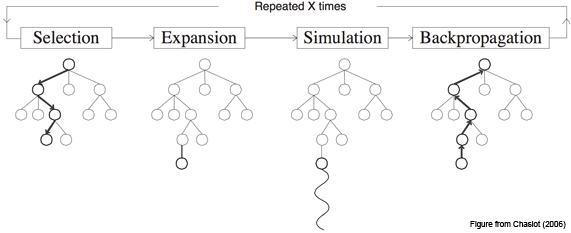
\includegraphics[scale=0.7]{rapport/images/graphics/mcts-algorithm.png}
            \caption{Monte Carlo tree search}
            \label{Monte_carlo_tree_search}
        \end{figure}
        
        
        
        \section{Game cloning}
        Cloning the game is a necessary procedure because when we have to act we have to simulate the game for us and for the other opponents. This operation allows us to keep the state of the game unchanged and pick up where we left off.
        To clone the game we tried to use two methods, one with an external library called \textbf{Gson} and the other one by using the \textbf{Java} built-in interface \textbf{Cloneable}. 
        We have chosen to use the second method because the Gson was not entirely working and the built-in was more advanced.
        
        \subsection{Gson library}
        
        The principle of the \textbf{Gson} library is to make a copy of the whole object even if it's containing other objects. In our case the object that enveloped the whole game is the class GameController and it is the one that we will copy. \\
        How does this method work ? The first thing we need to do is to make a deep copy (copy every nested object) of each object and \textbf{Gson} handles that very easily by transforming an object to JSON format. Once everything is copied we need to load the JSON data to convert them back into real objects with their respective parameters.
        
        \subsection{Built-in Cloneable implementation}
        
        \textbf{Cloneable} is an interface that is used to create an exact copy of an object. Every class used in Monte Carlo algorithm is implementing this interface (Player, Dice, Board, ...). It was necessary to implement the sequence of cloning for example when we clone the DiceSet it also clones each Dice inside. It was an important step because it created infinite loops, we had to be clever to make it work. \textbf{Cloneable} clone well primitives types stored in a class but not others objects so it was necessary to manually add the cloning of these objects.
        
        
        \section{Monte Carlo implementation}
        
        While building our algorithm, we realized that there were many possibilities and that our implementation was creating a stack overflow even though we were trying with few branches and depth. It was necessary to find a solution so we decided to change the type of choice during the simulation. The choices implemented in Monte Carlo of the game are random and do not follow the Monte Carlo algorithm.\\ \\
        As you can see in the figure \ref{Monte_carlo_tree_search}, a traditional algorithm creates a complete tree, but with our changes our algorithm creates a tree that looks like the figure \ref{Monte_carlo_SPBS}. This figure represents the tree behind a choice from our Monte Carlo. The root, representing the function call, will create 5 simulation branches. The first node of each branch is a temporary random choice and its child is a simulation of turns of the game with a depth of 2. In the simulation the die and action are randomly chosen and the other choices are default choices.\\ \\
        Once the algorithm is done with the branch for \textbf{Choice 1}, the choice with the best score is saved, and the branch \textbf{Choice 2} is explored. Upon finishing that branch, the scores of the first choice and of the choice from that branch will be compared, and the best one will be saved. These steps will be repeated until every branch is done.
        \\ \\
        
        
        \begin{figure}[H]
            \centering
            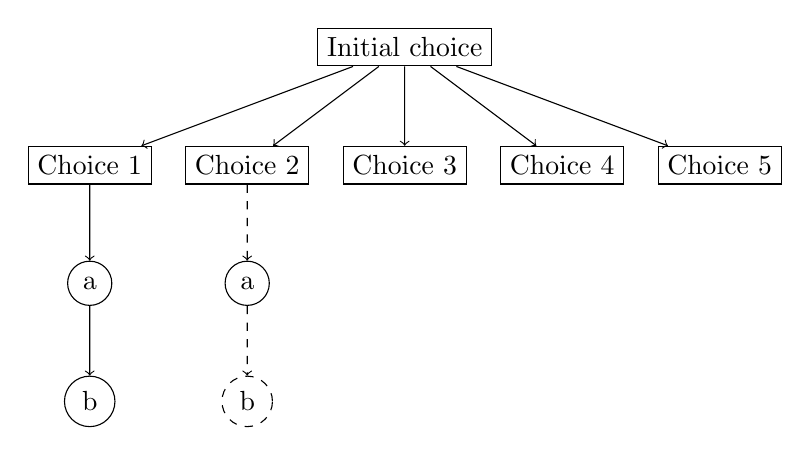
\begin{tikzpicture}[nodes={draw}, ->]
 
            \node{Initial choice}[sibling distance = 2cm]
            child { node {Choice 1} [circle]
                child {node{a}
                    child {node{b}
                        }}}
            child { node {Choice 2} [circle]
                child { node {a} [dashed]
                    child {node {b}}}}
            child { node {Choice 3}}
            child { node {Choice 4}}
            child { node {Choice 5}}
                ;
            \end{tikzpicture}
            \caption{Monte Carlo SPBS}
            \label{Monte_carlo_SPBS}
        \end{figure}


        \subsection{Hand initialization}
        
        During the guaranteed AI part, we saw that the initialization of the player's hand was important for the win-rate. Moreover it is out of any game loop so it seemed easier to start with it.\\
        At the beginning of the game, each player receives 9 cards. When it's an AI Monte Carlo's turn to receive them, we clone the board and the cards. The AI randomly chooses the arrangement of its hand and emulates the choice of the players after it. Then a game is simulated until the end, and this temporary choice with the associated prestige points at the end of the simulated game is saved.\\
        These operations are repeated for the number of connections given in the AI configuration.
        The temporary choice with the best prestige points is selected and returned.
        The real game resumes and the remaining players can initialize their hand.
        
        \subsection{Choosing a dice}
        
        Every time the player wants to choose a dice the algorithm will try several dice and see which one is the best to take at that moment of the game. We chose to make \textbf{Choose Dice} a unique strategy for Monte Carlo because it is a mandatory choice a player will have to make at one point.\\
        When the Monte Carlo player chooses a die the game is cloned and we emulate the random temporary choice of the die. For the players who have to play afterwards we also emulate their choices.The players make their turns and we simulate as many game turns as the depth indicated in the configuration. That is repeated for the number of branches written in the configuration. Then, just like for the initialization, we keep the best temporary choice.
        
        \subsection{Generating the player's actions}
        
        For this part the player's moves for the turn are randomly generated. Basically this method will try multiple moves. For instance we could invoke 3 cards and activate 1 card in the current turn but we will actually try to summon only 1 cards, or none, etc. in a random way. Then we will check which choice was the best to make at the end of the tree search.
        To make this possible we had to create a specific class called MonteCarloTurnLoop which extends PlayerTurnLoop to override how a turn of a Monte Carlo player works and adapt it to our algorithm. In comparison a basic player will make an action until he doesn't want to do anything while Monte Carlo will generate a list of the best actions and then execute it.
        \newpage
        \section{Different versions of Monte Carlo}
        
        \subsection{Random}
        
        This version is a totally randomized algorithm, this means that all the choices the AI will make are randomly tested. For example when the AI wants to crystallize an energy, it will first try to crystallize an earth energy, it can try with fire one, or even with no energy, that choice being random.
        
        \subsection{Heuristic}
        
        After trying a fully random Monte Carlo we decided to add an heuristic to get better results. The heuristic that we used is based on the previous guaranteed AI, with the composed strategies. We still have random choices in this version, particularly in the generation of the moves, the choice of a die and the initialization of the hand like previously stated. For all the other AI choices we used the heuristic from our best guaranteed AI to make it smarter, for example when it comes to summoning a card, we will use the composed strategy.
        
        \section{Performance}
        
        We did some performance testing to see which parameter values are the best for the Monte Carlo Random through our statistics server. For each branch from 1 to 20 and for each depth from 1 to 15 and for each action from 1 to 20, we tested each combination of the parameters on 100 games each time and we took the 3 best win-rates.\\
        On the figures \ref{perf_random} and \ref{perf_monte_carlo_compose}, each point represents an average per observed category. This average is calculated on 100 games with unique parameters.\\
        Both figures are periodic and it can be explained by the rotation of the parameters, when the number of actions is low all curves decrease. With the best parameters, the win rate and the curves for the prestige points and the points of cards are high but the AI does not summon enough cards, so it accumulates too many penalties. We think the problem is that the AI prioritize crystals and leaves energies, and without energies it can't invoke many cards. 
        
        \subsection{Monte Carlo Random}
        
        The figure \ref{perf_random} shows the best results we have for the random Monte Carlo against the random strategy, so the best combination of parameters is 6 branches, depth of 12 and 17 actions.\\
        
        As you can see in the figure \ref{perf_monte_carlo_random_against}, our AI Monte Carlo Random is quite good against not composed AI like Activate, Malus... But although it as 71\% of victory against the random AI, it isn't as good as our composed AI.
        Moreover when we look at the matches between Monte Carlo and the composed AIs, it is obviously not really good with a win-rate below 20\%.
        
        The fact that Monte Carlo is not very good against our best guaranteed AI can be explained by its nature. Monte Carlo is an AI which explores possibilities in the game, but Seasons is a game with a lots of different possibilities and a little choice can change many things. That being said, we decided to keep an AI which take decisions quickly which naturally impacts the research. In order to be faster the AI explores less possibilities and by that fact is less efficient. 
        
        \begin{figure}[H]
            \centering
            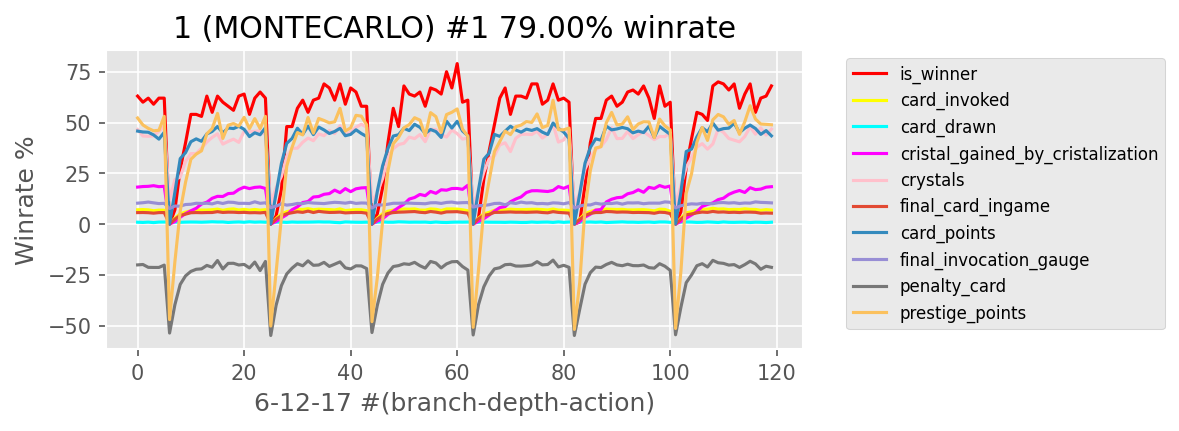
\includegraphics[scale=0.75]{rapport/images/graphics/1 (MONTECARLO)-1555-1.png}

            \caption{Monte Carlo random best parameters \#1}
            \label{perf_random}

        \end{figure}
        
        \begin{figure}[H]
            \centering
            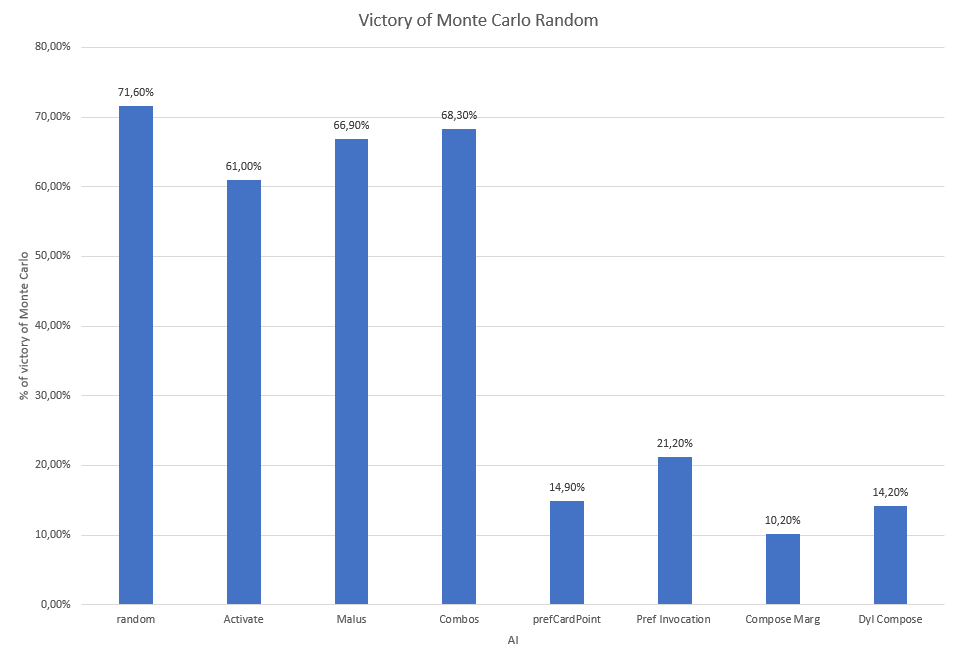
\includegraphics[scale=0.45]{rapport/images/graphics/fight_MT_random.png}
            \caption{Monte Carlo random percentage of victory against other AI}
            \label{perf_monte_carlo_random_against}

        \end{figure}
        
        \subsection{Monte Carlo Heuristic}
        
        As you can see in the figure \ref{perf_monte_carlo_compose} we have a 39\% win-rate against one of the best guaranteed strategies which is \textit{PrefCardPoints}. The best parameters that we found for the heuristic are the following: 5 branches, depth of 4 and 16 actions.\\
        
        The performances of Monte Carlo Compose with these parameters against other strategies are visible in the figure \ref{perf_monte_carlo_compose_against}. The AI wins by a large margin against the strategies Random, Activate, Malus and Combos. We can also see better results than Monte Carlo Random for the strategies Pref Invocation, Pref Card Point, Compose Marg and Compose Dyl. As this AI is based on Compose Marg, we could hope to win at least against Pref Invocation and Pref Card Point. We think the poor performances are caused by the initialization of the hand, since choices are random and during the simulation the choices of the other players are randomly emulated.
        
        
        
        \begin{figure}[H]
            \centering
            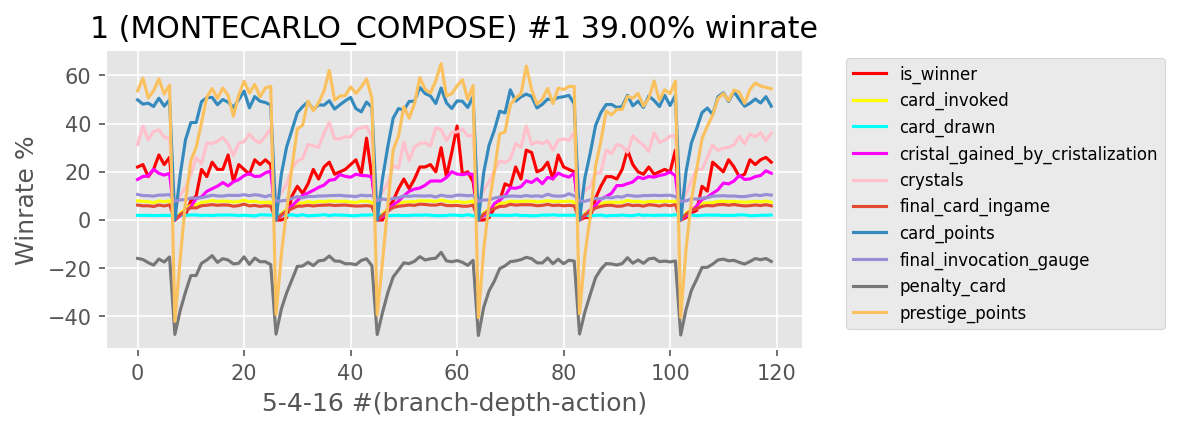
\includegraphics[scale=0.75]{rapport/images/graphics/1_MONTECARLO_COMPOSE-1136-1.png}
            \caption{Monte Carlo heuristic best parameters \#1}
            \label{perf_monte_carlo_compose}

        \end{figure}
        
        \begin{figure}[H]
            \centering
            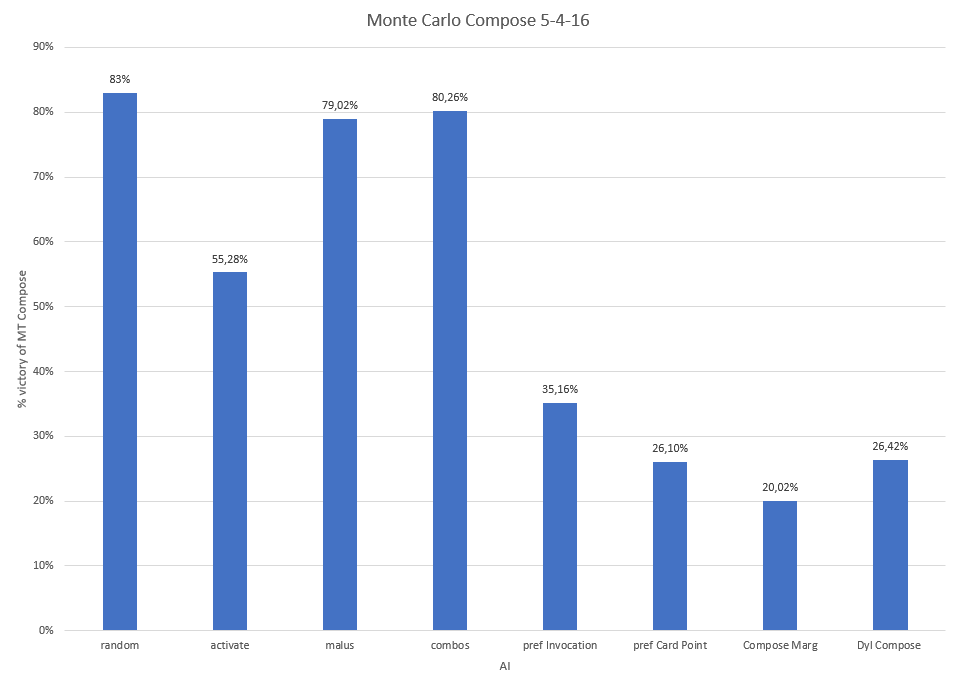
\includegraphics[scale=0.45]{rapport/images/graphics/fight_MT_COMP_5_4_16.png}
            \caption{Monte Carlo heuristic percentage of victory against other AI}
            \label{perf_monte_carlo_compose_against}

        \end{figure}
        
   
        
        


        
    